\documentclass[aspectratio=169,usenames,dvipsnames]{beamer}
\beamertemplatenavigationsymbolsempty
% \documentclass{beamer}

% UNCOMMENT FOR HANDOUTS
% \usepackage{pgfpages}
% \pgfpagesuselayout{2 on 1}[landscape,letterpaper,border shrink=5mm]
% \setbeameroption{show notes}

\mode<presentation>
\usetheme{Boadilla}
\usecolortheme{spruce}
\usepackage{../../LizStyle,ulem}
\usepackage{color}
\usepackage[color,matrix,arrow]{xy}
% \input xy
% \xyoption{all}
\usepackage{tikz}
\usepackage{tikz-cd}
\tikzset{commutative diagrams/diagrams={ampersand replacement=\&}}

\AtBeginSection{\frame{\sectionpage}}


% ==========Command for putting comments and removing them=======
% Visible:
\newcommand{\InstructorNotes}[1]{\textit{\color{orange}#1}}
\newcommand{\InstructorList}[1]{
\begin{itemize}
	\color{orange}
	#1
\end{itemize}
}
% Removed:
% \renewcommand{\InstructorNotes}[1]{}
% \renewcommand{\InstructorList}[1]{}


\newcommand{\bvfill}{\vskip0pt plus 1filll}

\usepackage{multimedia}
\usepackage{graphbox}

% \usepackage{algpseudocode}


\newcommand{\Reeb}{\textbf{Reeb}}
\newcommand{\Rtopc}{\textbf{Rtopc}}
% \newcommand{\RR}{\mathcal{R}}

\newcommand{\Set}{\textbf{Set}}
\newcommand{\Vect}{\textbf{Vect}}
\newcommand{\Top}{\textbf{Top}}
\newcommand{\Int}{\textbf{Int}}


\graphicspath{ {Figures/} {../../Figures/} }



\begin{document}
%\pdfoptionpdfminorversion 5
%\logo{\includegraphics[height=1.5cm]{dukeshield.pdf}}
\title[Review day]{Test 3 review day}
\subtitle{CMSE 381}
\date{Fri, Nov 21, 2025}



\institute[MSU-CMSE]{Michigan State University\\
			::\\
          Dept of Computational Mathematics, Science \& Engineering}
\author[Dr.~Zhang]{Prof.~Mengsen Zhang}

\begin{frame}
 \titlepage


\end{frame}
%--------------------------
\begin{frame}[c]{Announcements}

\begin{columns}

\column{.60\textwidth}
\centering

	Announcements: 
	\begin{itemize}
		\item midterm \# 3 on Monday
		\item Bonus code portfolio assignment due Nov 26 on D2L.
		\item Final Project submission on D2L. Due Dec 5. 
		% \item Student Perception of Learning Survey (SPLS): \href{https://go.blueja.io/34gZ5pyBAky23zqp9vjplA}{Please fill out this}
	\end{itemize}
	% 
\includegraphics[width=.3\textwidth]{SPLS_S25-001.png}
\end{columns}

\end{frame}
%--- Next Frame ---%
\begin{frame}[c]{Based on the questions submitted}

\begin{columns}
\column{.5\textwidth}
\centering
\begin{itemize}
	\item Cubic spline math
	\item Bagging and random forests
	\item SVM kernels
	\item Convolutional and softmax output
\end{itemize}
\column{.4\textwidth}
\centering

\end{columns}

\end{frame}
%--- Next Frame ---%
%==========
\section{Cubic Splines}
%==========

% ---- Next Frame --- %
\begin{frame}[t]{Cubic splines}

\begin{columns}
\column{.45\textwidth}
\centering

\begin{itemize}
	\item Fit piecewise polynomial
	\item Require continuity at knots
	\item Require the first and second derivatives to be continuous at knots
\end{itemize}
\InstructorList{
  \item Now we have smooth joins
	\item This is called a "cubic spline"
	\item 8 original degrees of freedom, plus three constraints (continuous, 1st deriv continuous, 2nd deriv continuous) leaves 5 degrees of freedom
	\item cubic spline with $K$ knots uses $4+K$ degrees of freedom
}
\column{.45\textwidth}
\centering
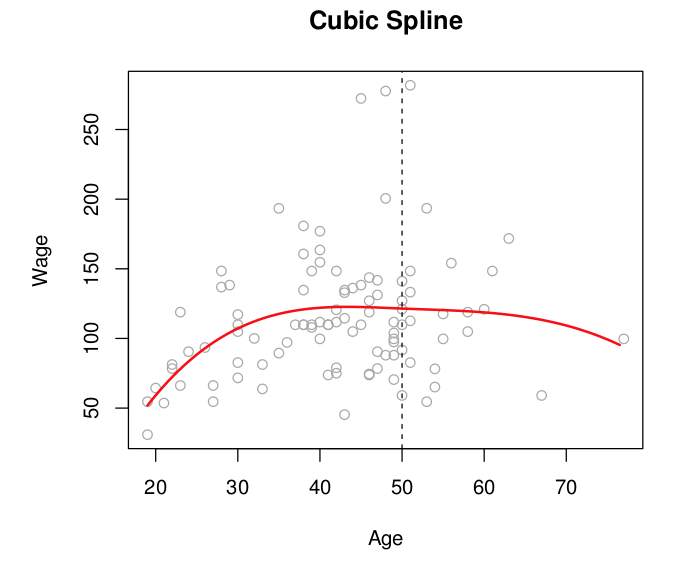
\includegraphics[width = \textwidth, align = c]{Fig7-3c}

Test your understanding: \href{https://PollEv.com/multiple_choice_polls/bkj0zshpQHzhiwM3UXroS/respond}{PollEv}
\end{columns}

\end{frame}
%--- Next Frame ---%
{
\setbeamercolor{background canvas}{bg=Apricot!25}
\begin{frame}[t]{Example}
\begin{columns}
\column{.45\textwidth}
\centering
We have the following piecewise cubic polynomial: 
\begin{equation*}
	f(x) = 
	\begin{cases}
		2+x+x^{2}+0.1x^{3} & x \leq 1 \\
		b_0 + b_1 x + b_2 x^2 -x^3 & x > 1
	\end{cases}
\end{equation*}
What are $b_1$, $b_1$, and $b_2$ to make this a cubic spline?
\column{.45\textwidth}
\centering
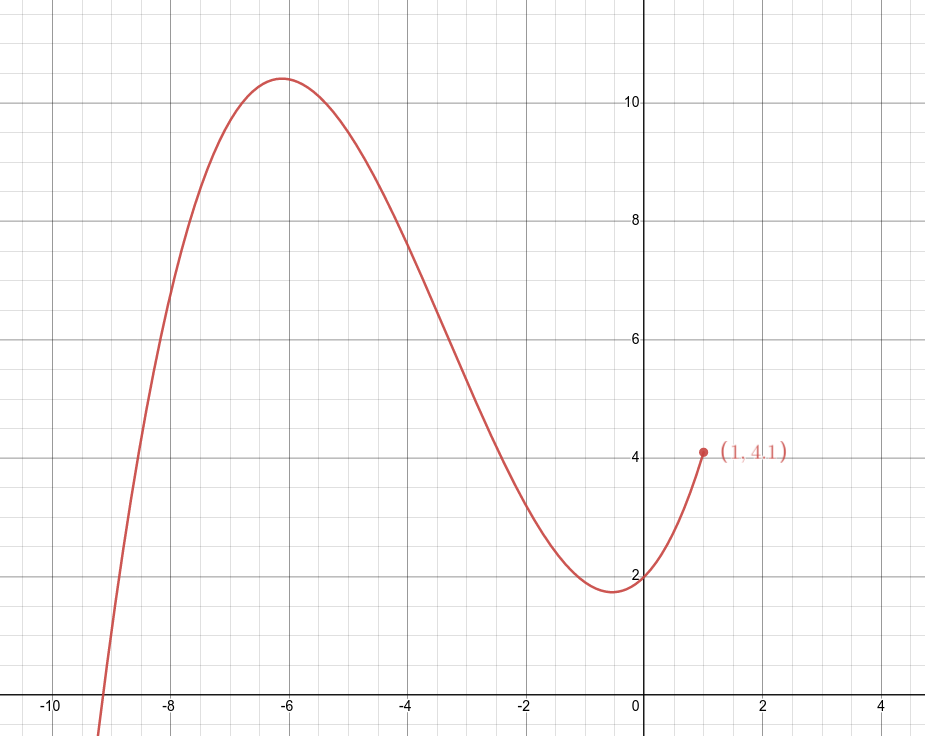
\includegraphics[align = c, width = \textwidth]{SplineMatchingExample.png}

\end{columns}

\bvfill
 Check your answers: \href{https://www.desmos.com/calculator/kbm0zivqco}
{www.desmos.com/calculator/kbm0zivqco}
\end{frame}
}
%--- Next Frame ---%
{
\setbeamercolor{background canvas}{bg=Apricot!25}
\begin{frame}[t]{More space for work}

\begin{columns}
\column{.45\textwidth}
\centering
	\begin{equation*}
		f(x) = 
		\begin{cases}
			2+x+x^{2}+0.1x^{3} & x \leq 1 \\
			b_0 + b_1 x + b_2 x^2 -x^3 & x > 1
		\end{cases}
	\end{equation*}
	\InstructorNotes{
Instructor tool for generating solution while messing with $b_3$: \url{https://www.desmos.com/calculator/5prmps9cuo}
	}
\column{.45\textwidth}

\centering
\InstructorNotes{
	\begin{equation*}
		f(x) = 
		\begin{cases}
			2+x+x^{2}+0.1x^{3} & x \leq 1 \\
			3.1 + -2.3 x + 4.3 x^2 -x^3 & x > 1
		\end{cases}
	\end{equation*}
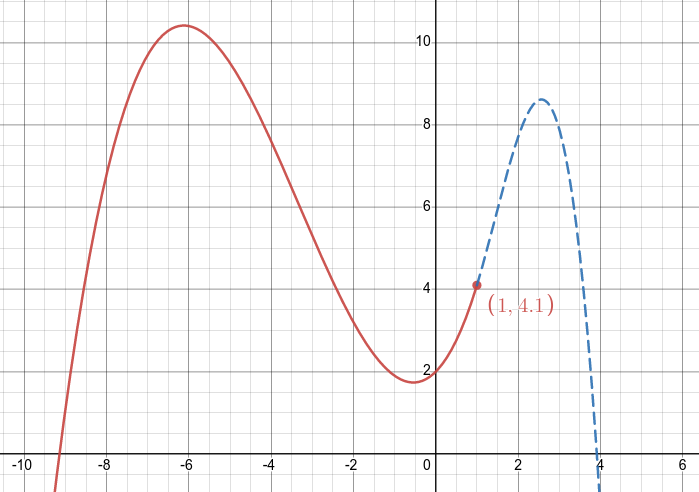
\includegraphics[align = c, width = .6\textwidth]{SplineMatchingExample-Soln}
	}

\end{columns}
\end{frame}
}
%--- Next Frame ---%

\begin{frame}[t]{Notes on cubic splines }

\begin{columns}
\column{.45\textwidth}
\centering

\InstructorList{
  \item Human eyes can't detect the discontinuities so often cubic splines are a good way to go
	\item Still have problem of high variance at the outer range of predictors (big or small $X$)
	\item \textit{Natural spline:} regression spline plus boundary constraints where function is required to be linear at the boundary
}

\column{.45\textwidth}
\centering

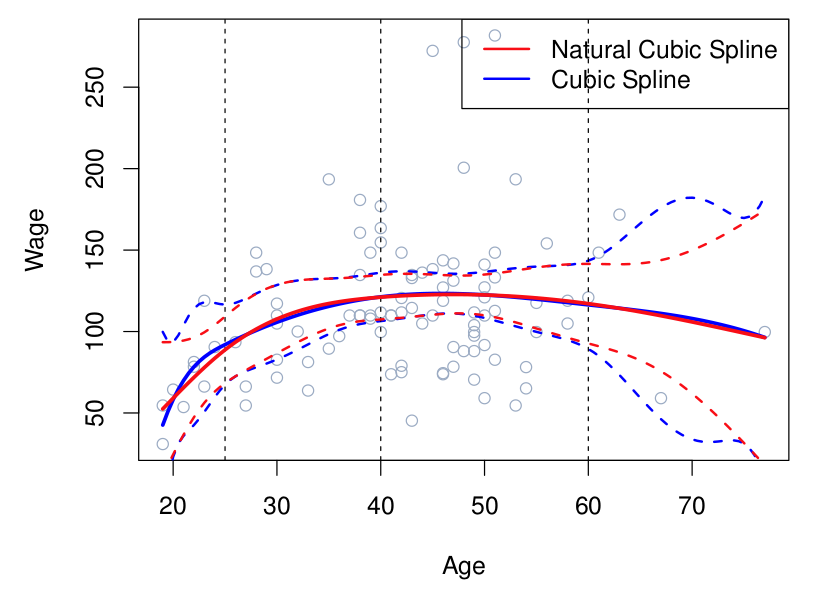
\includegraphics[width = \textwidth]{Fig7-4}
\end{columns}

\end{frame}

%--- Next Frame ---%
% \begin{frame}[t]{How many knots to use?}
% {When in doubt, Cross-Validate.}
% \begin{columns}
% \column{.45\textwidth}
% \centering

% \InstructorList{
% 	\item need to know knot is a flexibility parameter, hence all the bias-variance trade-off stuff applies.
%   \item Do CV ($k$-fold probably) on data for each number of knots
% 	\item Figure at right is the MSE resulting from 10-fold CV
% 	\item Note that clearly linear is not enough, after that 3-4 degrees of freedom for the cubic spline are enough
% }

% \column{.45\textwidth}
% 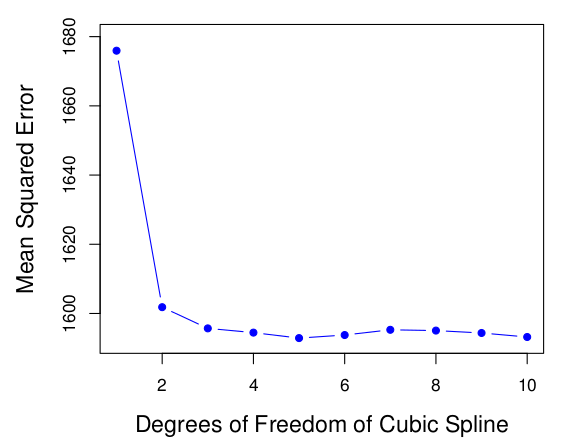
\includegraphics[width = \textwidth]{Fig7-6b}
% \centering

% \end{columns}
% \end{frame}

%% ======== bagging and random forests ========
\section{Bagging and Random Forests}

\begin{frame}[t]{Use ensemble of trees to reduce variance}

\begin{columns}
\column{.45\textwidth}
% \centering
% Averaging a set of observations reduces variance:
% \begin{itemize}
% 	\item $n$ independent observations $Z_1,\cdots, Z_n$ each with variance $\sigma^2$
% 	\item Variance of the mean $\bar Z$ is $\sigma^2/n$
% \end{itemize}

\textbf{Want to do (but can't):} \\
Build separate models from independent training sets, and average resulting predictions:
\begin{itemize}
	\item $\hat f^1(x), \cdots, \hat f^B(x)$ for $B$ separate training sets
	\item Return the average
	\begin{equation*}
		\hat f_{avg}(x) = \frac{1}{B} \sum_{b=1}^B \hat f^b(x)
	\end{equation*}

\end{itemize}
\InstructorList{
  \item Decreases variance, but not practical
}

\column{.45\textwidth}
% \centering

\textbf{Boostrap modification:}
\begin{itemize}
	\item Work with fixed data set
	\item Take $B$ samples from this data set (with replacement)
	\item Train method on $b$th sample to get $\hat f^{*b}(x)$
	\item Return average of predictions (regression)
	\begin{equation*}
		\hat f_{bag}(x) = \frac{1}{B} \sum_{b=1}^B \hat f^{*b}(x)
	\end{equation*}
	or majority vote (classification)
\end{itemize}



\end{columns}

\end{frame}
%--- Next Frame ---%

\begin{frame}[t]{Tree version}
	\centering
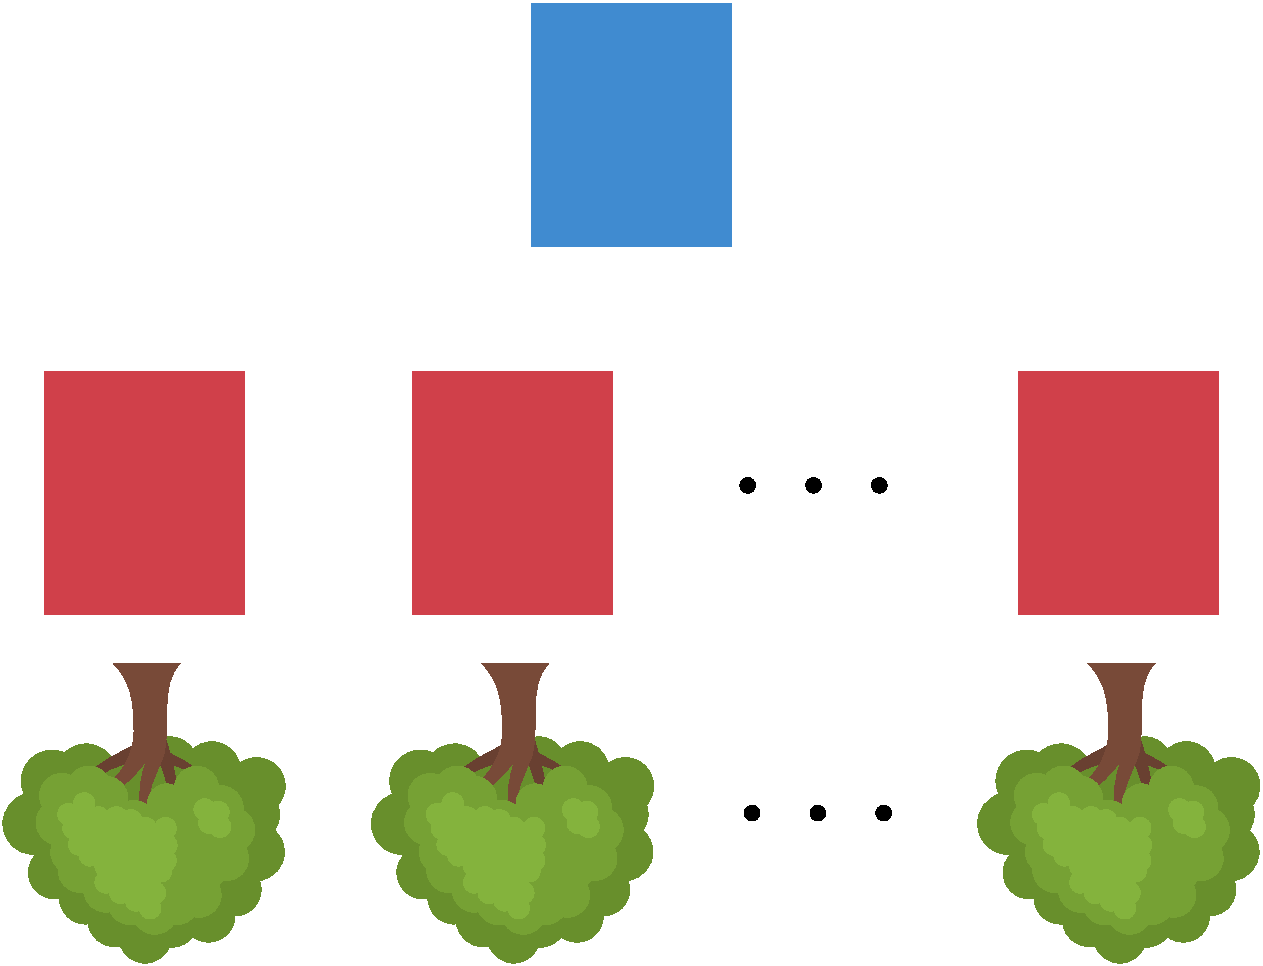
\includegraphics[width = .6\textwidth, align = c]{TreeBaggingCartoon}
\InstructorNotes{
	\begin{minipage}
		{.35\textwidth}
		\InstructorList{
		\item Blue is original data set $X:n \times p$ 
		\item Red are the subsampled  data sets 
		\item Build a tree from each 
		\item Get prediction from each, return the average
		}
	\end{minipage}
}
\end{frame}
%--- Next Frame ---%
\begin{frame}[c]{Prediction on new data point }
\InstructorNotes{New data point goes in, run through each tree, average outputs}
\centering
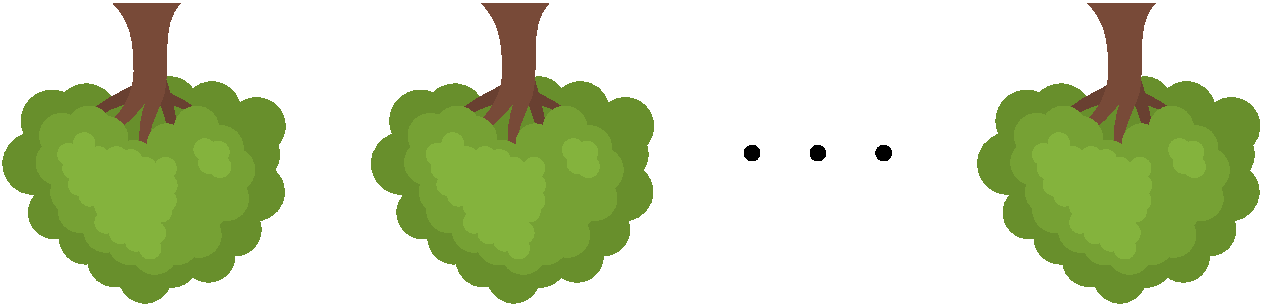
\includegraphics[width = .6\textwidth]{TreeBaggingCartoon-OnlyTrees}

\end{frame}

%--- Next Frame ---%
\begin{frame}[t]{Out of Bag Error Estimation}

\begin{columns}
\column{.45\textwidth}
\centering
\begin{itemize}
	\item On average, bootstrap sample uses about 2/3 of the data \InstructorNotes{We did this homework problem a while ago I think? Ch 5, Ex. 2}
	\item Remaining observations not used are called \textit{out-of-bag} (OOB) observations
	\item For each observation, run through all the trees where it wasn't used for building
	\item Return the average (or majority vote) of those as test prediction! rather law of large number
	\item Bootstraped version of LOOCV.
\end{itemize}
\column{.45\textwidth}
\centering
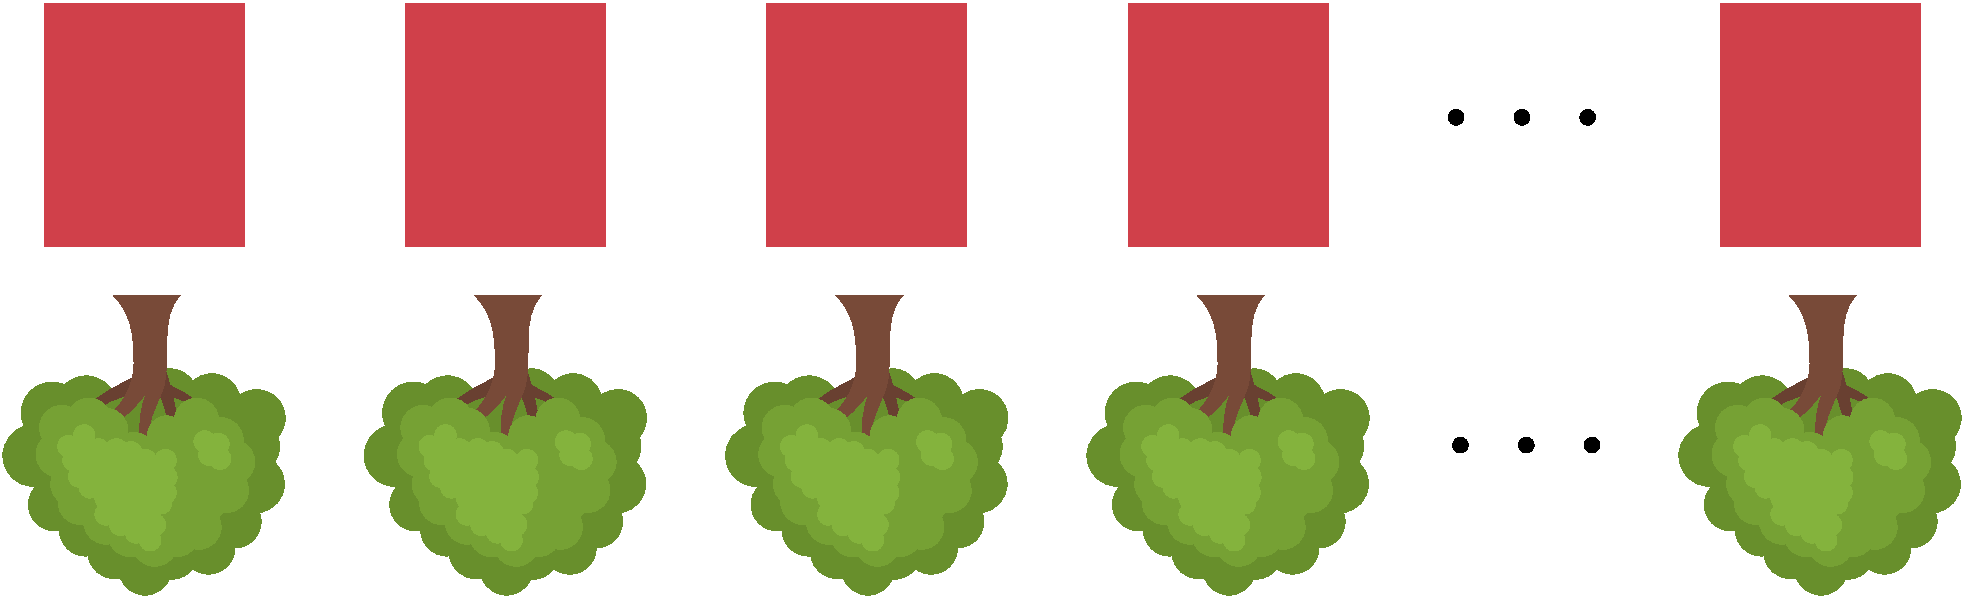
\includegraphics[width = \textwidth]{TreeBaggingCartoon-MoreTrees}
\end{columns}

\end{frame}

%--- Next Frame ---%

\begin{frame}[t]{Random Forests}

\begin{columns}
\column{.45\textwidth}
\centering
\begin{itemize}
	\item Goal is to decorrelate the bagged trees:
	\begin{itemize}
		\item If there is a strong predictor, the first split of most trees will be the same
		\item Most or all trees will be highly correlated
		\item Averaging highly correlated quantities doesn't decrease variance as much as uncorrelated
	\end{itemize}
\end{itemize}
\column{.45\textwidth}
\centering
\begin{itemize}
	\item The random forest fix:
	\begin{itemize}
		\item Each time a split is considered, only use a random subset of $m$ the predictors
		\item Fresh sample taken every time
		\item Typically $m \approx \sqrt p$
		\item On average, $(p-m)/p$ of splits won't consider strong predictor
		\item $m = p$ gives back bagging
	\end{itemize}
\end{itemize}
\end{columns}

\end{frame}



\section{SVM Kernels}
%--- Next Frame ---%


\begin{frame}[t]{The kernel - replacing global coordinate with local similarity}

\begin{columns}
\column{.45\textwidth}
\centering
\begin{equation*}
	K(x_i,x_i')
\end{equation*}
\InstructorList{
	\item $K(x_i,x_i')$ can be thought of as similarity function.
  	\item An example is inner product $\langle x, x_i \rangle$ will be talked about in more detail on the next slide.
	\item $\langle x, x_i \rangle$ is known as a linear kernel
	% \item near kernel essentially quantifies the similarity of a
% pair of observations using Pearson (standard) correlation
}

\column{.45\textwidth}
\centering
$y_i f(x_i)\geq M(1-\epsilon_i)$, where
\begin{equation*}
	f(x) = \beta_0 + \sum_{j \in \mathcal{S}}\alpha_i K(x,x_j)
\end{equation*}

\InstructorList{
  \item The function defined is as above with whatever choice of $K$
  
	\item When the support vector classifier is combined with a non-linear kernel the resulting classifier is 	known as a support vector machine.
}

\end{columns}

\end{frame}

%--- Next Frame ---%

\begin{frame}[t]{SVC via inner products}
	\centering
%   $f(x) = \beta_0 + \beta_1x_1 + \cdots + \beta_px_p = \beta_0 + \langle \beta, x\rangle$
\begin{equation*}
	f(x) = \beta_0 + \sum_{i=1}^n \alpha_i \langle x, x_i \rangle
\end{equation*}

\begin{equation*}
	f(x) = \beta_0 + \sum_{i\in\mathcal{S}} \alpha_i \langle x, x_i \rangle
\end{equation*}

\begin{columns}
\column{.45\textwidth}
\centering

\InstructorList{
	\item Via some magic, there are coefficients $\alpha_i$ which give the linear support vector classifier 
	\item In this notation, the $x_i$'s are all the training points 
	% \item How to actually get it is outside the scope of this class
	% \item To estimate the paramters $\alpha_1,\cdots,\alpha_n$ and $\beta_0$, need $\binom{n}{2} = n(n-1)/2$ inner products $\langle x_i,x_{i'} \rangle$
}

\column{.45\textwidth}
\centering
\InstructorList{
  \item How to actually get it is outside the scope of this class
  \item To estimate the paramters $\alpha_1,\cdots,\alpha_n$ and $\beta_0$, need $\binom{n}{2} = n(n-1)/2$ inner products $\langle x_i,x_{i'} \rangle$
  \item BUT, $\alpha$ is only non-zero for support vectors. so actually few terms
}


\end{columns}

\end{frame}

%--- Next Frame ---%


\begin{frame}[t]{The kernel - more generally}

\begin{columns}
\column{.45\textwidth}
\centering
\begin{equation*}
	K(x_i,x_i')
\end{equation*}
\InstructorList{
  \item Swap out my inner product $\langle x, x_i \rangle$ for something potentially more complicated
	\item $\langle x, x_i \rangle$ is known as a linear kernel
	% \item near kernel essentially quantifies the similarity of a
% pair of observations using Pearson (standard) correlation
}

\column{.45\textwidth}
\centering
\begin{equation*}
	f(x) = \beta_0 + \sum_{i \in \mathcal{S}}\alpha_i K(x,x_i)
\end{equation*}

\InstructorList{
  \item The function defined is as above with whatever choice of $K$
  \item $K(x_i,x_i')$ can be thought of as similarity function.
	\item When the support vector classifier is combined with a non-linear kernel the resulting classifier is 	known as a support vector machine.
}

\end{columns}

\end{frame}
%--- Next Frame ---%
\begin{frame}[t]{A polynomial kernel}
\begin{equation*}
	K(x_i,x_{i'}) = \left(1 + \sum_{j=1}^p x_{ij}x_{i'j} \right)^d
\end{equation*}
\begin{columns}
\column{.45\textwidth}
\centering

\InstructorList{
  \item much more flexible decision boundary.
	\item amounts to fitting a support vector
classifier in a higher-dimensional space involving polynomials of degree $ d$,
rather than in the original feature space.
\item Right: degree 3 polynomial kernel

}

\column{.35\textwidth}
\centering
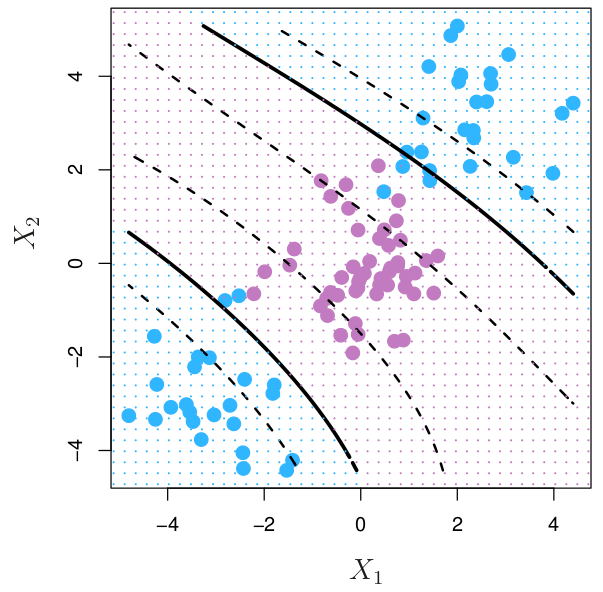
\includegraphics[width = \textwidth]{Fig9-9a}
\end{columns}

\end{frame}
%--- Next Frame ---%


\begin{frame}[t]{A radial kernel}
\begin{equation*}
	K(x_i,x_i') = \exp \left( -\gamma \sum_{j=1}^p(x_{ij} - x_{i'j})^2 \right)
\end{equation*}
\begin{columns}
\column{.45\textwidth}
\centering

\InstructorList{
%   \item Draw picture of circular values around a point
  \item this is essentially a gaussian kernel
	\item big distance makes $\sum (x_{ij}-x_{i'j})^2$ big, but then $e^{-big}$ is tiny.
	\item In $f(x)$, this means that $x_i$ plays little role if it's far away.
	\item Radial kernel has local behavior
}

\column{.35\textwidth}
\centering
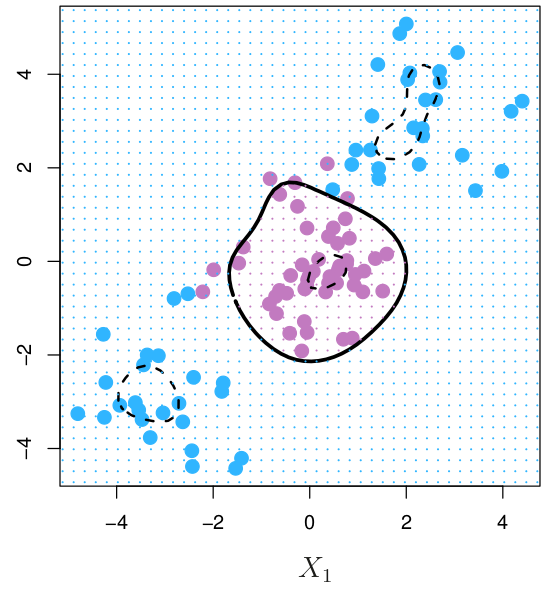
\includegraphics[width = \textwidth, align = c]{Fig9-9b}
\end{columns}

\end{frame}

%==========
\section{Convolutional Neural Networks and softmax output}
%==========

%--- Next Frame ---%

\begin{frame}[t]{CNN}

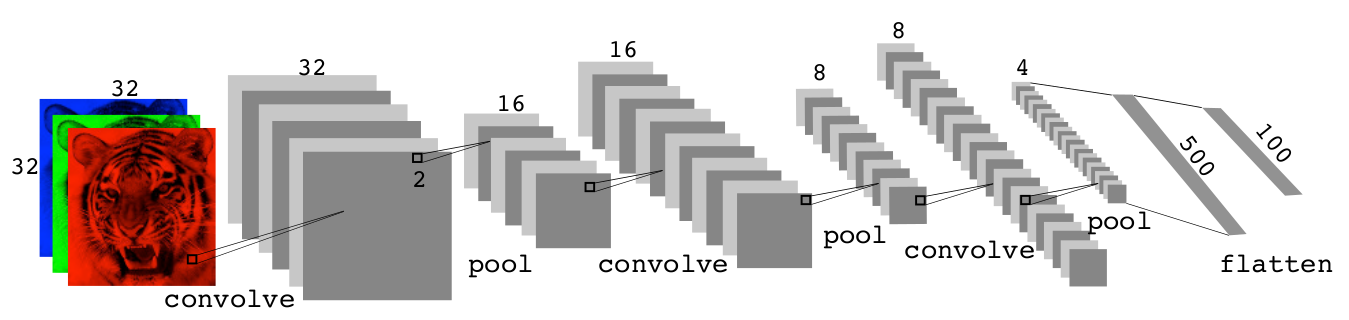
\includegraphics[width = \textwidth, align = c]{Fig10-8}
\begin{columns}
\column{.45\textwidth}
\centering
\footnotesize
\InstructorList{
  \item Start with three channels
	\item conv layer -- extract spatial features via convolution with learned filters
	\item Next is max pool layer, spatial coarse-graining
	\item convolve \& pool several more times
	% \item Can repeat several convolves before pool, this effectively increases the dimension fo the feature
}

\column{.45\textwidth}
\centering
\footnotesize
\InstructorList{
	\item Since size of image decreased, we increase number of filters in the next convolve layer to compensate
  \item Flattened, then fed into 1 or more fully-connected layers
	\item Last is softmax activation for the 100 classes
}

\end{columns}
\bvfill
\url{https://poloclub.github.io/cnn-explainer/}

\end{frame}

%--- Next Frame ---%

\begin{frame}[t]{Convolution layer }
	{Convolution Filter}

\begin{columns}
\column{.45\textwidth}
\centering
Original Image:
\begin{equation*}
	\begin{bmatrix}
		a & b & c\\
		d & e & f \\
		g & h & i\\
		j & k & l
	\end{bmatrix}
\end{equation*}

Convolution filter:
\begin{equation*}
	\begin{bmatrix}
		\alpha & \beta \\
		\gamma & \delta
	\end{bmatrix}
\end{equation*}
\column{.45\textwidth}
\centering
Convolved Image
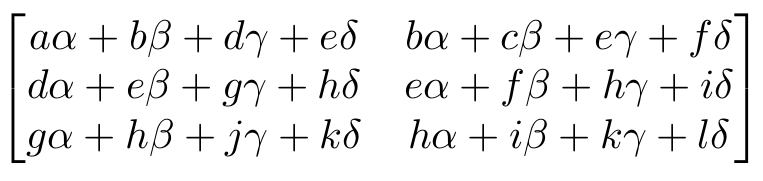
\includegraphics[width = \textwidth, align = c]{CNN-ConvolvedImage.png}

\InstructorNotes{Note we are just doing inner product here, which measure(ish) similar}
\end{columns}

\end{frame}
%--- Next Frame ---%
\begin{frame}[t]{Convolution Filter Example}

\begin{columns}
\column{.25\textwidth}
\centering
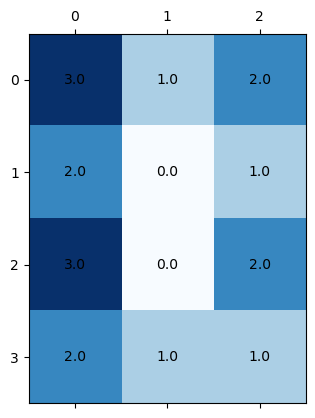
\includegraphics[width = \textwidth, align = c]{CNN-examplematrix}
% 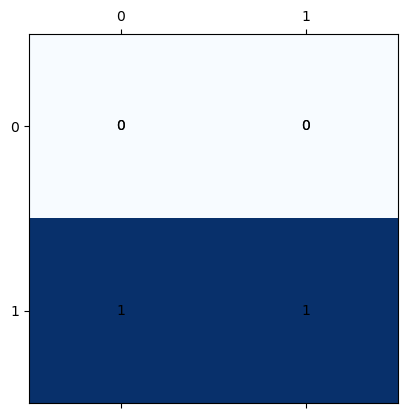
\includegraphics[width = .5\textwidth, align = c]{CNN-examplematrix-Mask}

Filter:
\begin{equation*}
	\begin{bmatrix}
		0 & 1 \\
		0 & 1
	\end{bmatrix}
\end{equation*}
\column{.45\textwidth}
\centering

\InstructorList{
\item $\begin{bmatrix}
	1 & 3 \\
	0 & 3 \\
	1 & 3
\end{bmatrix}$
\item Convolved image highlights regions that resemble the convolution filter. 
\item Conv or filtering is traditional signal processing, but in CNN the filter is learned (mentioned again later)
\item Note that the result is smaller than original
}
\end{columns}
\end{frame}


%--- Next Frame ---%
\begin{frame}[t]{Convolution filter: Bigger example}

	\centering
\begin{columns}
\column{.6\textwidth}
\centering
	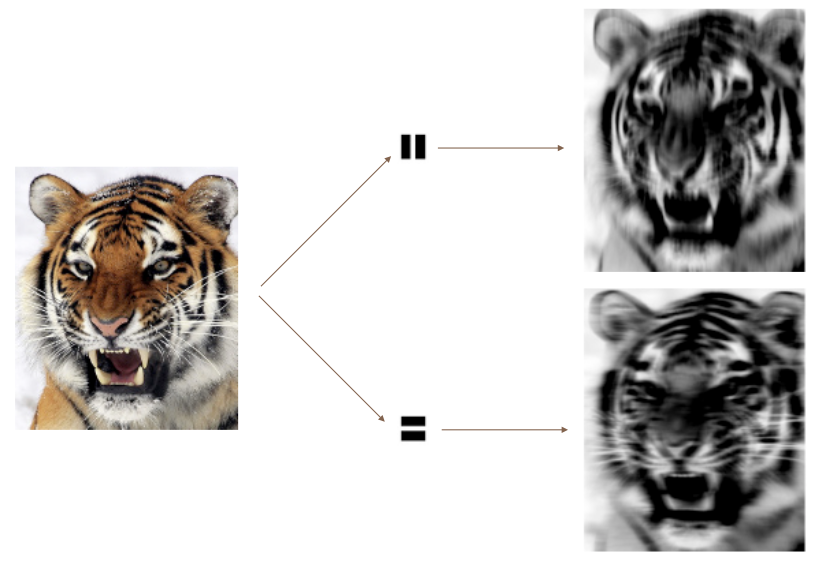
\includegraphics[width = \textwidth, align = c]{Fig10-7}

\column{.35\textwidth}
\centering
\InstructorList{
  \item 192x179 image of tiger
	\item Convolution filters are 15x15 images with mostly zero (black) narrow strip of ones (white)
	\item Highlights areas of the tiger that resemble the filter
}

\end{columns}

\end{frame}

%--- Next Frame ---%

\begin{frame}[t]{Pooling layers}

\begin{columns}
\column{.45\textwidth}
\centering
\InstructorList{
  \item Condense a large image into a smaller summary image
	\item Lots of options, but max pooling is common:
	\item For each 2x2 non-overlapping block of pixels, get a single new pixel with the maximum value from the block
	\item Provides location invariance: so long as large value in one of the four pixels, the whole block registers as a large value
}

\column{.45\textwidth}
\centering
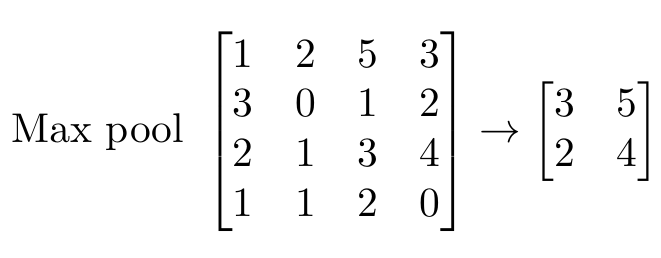
\includegraphics[width = \textwidth, align = c]{Eq10-3-2.png}
\end{columns}

\end{frame}


\begin{frame}[t]{The last column for classification: Softmax}

	\begin{columns}
	\column{.25\textwidth}
	\centering
	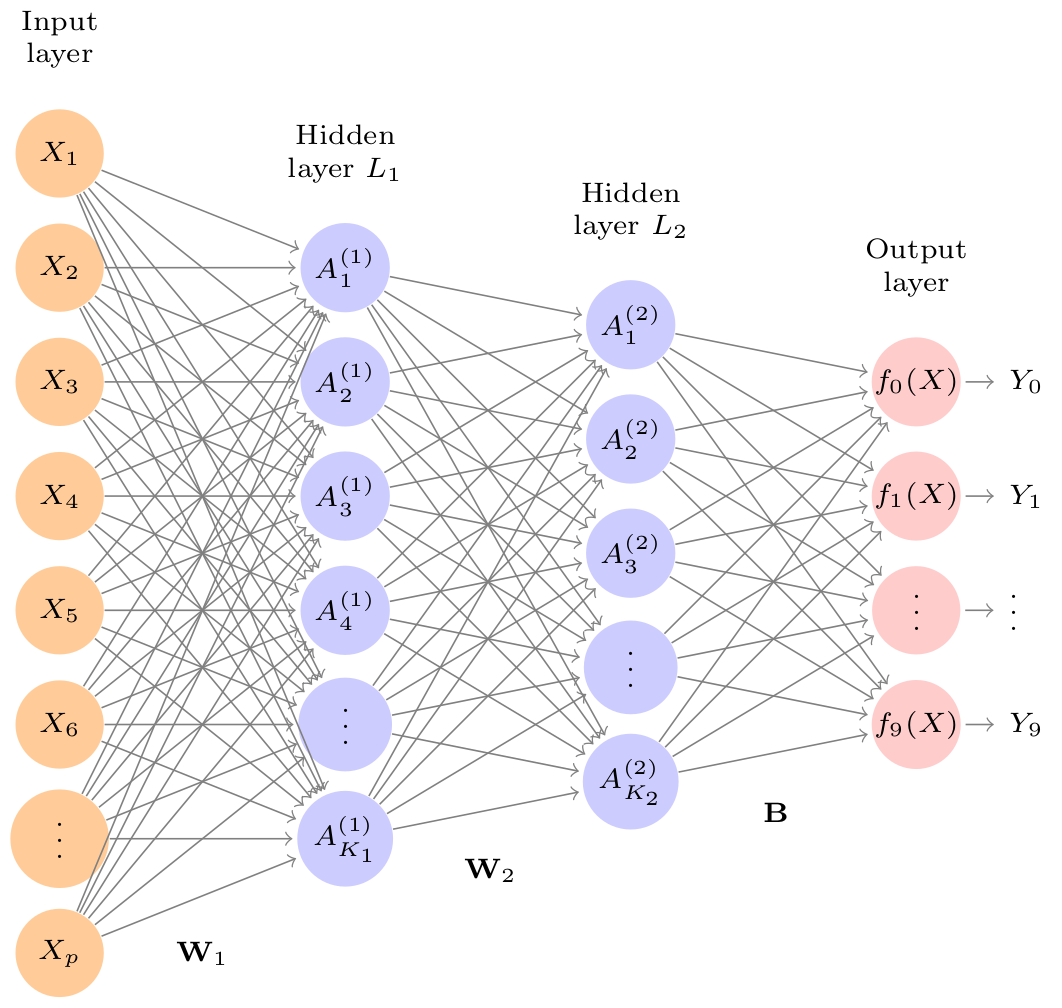
\includegraphics[width = \textwidth, align = t, clip, trim = 500 0 0 0]{Fig10-4}
	\column{.45\textwidth}
	\centering
	% 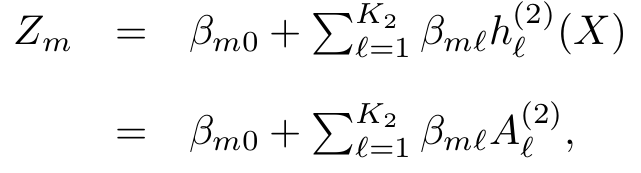
\includegraphics[width = \textwidth, align = c]{Eq10-12}
	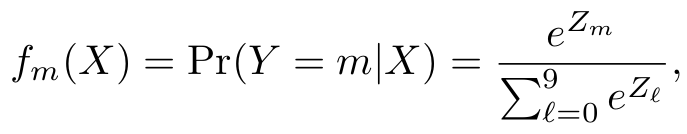
\includegraphics[width = \textwidth, align = t]{Eq10-13}
	\InstructorList{
	%   \item Doing linear combo of inputs to get 10 different outputs
		\item Want this to act like a probability.
		\item Answer is to use the softmax activation function $f_m(X)$
		\item Values are non-negative 
		\item Values sum to 1
		\item Return class with highest probability
	}
	
	
	\end{columns}
	
	\end{frame}


%-----------end frame------------

\end{document}
